\documentclass[fleqn]{article}
\usepackage[margin=3cm]{geometry}   % shrink margins
\usepackage[margin=3cm]{caption}   % shrink captions
\usepackage{amsmath}    % math equation environments
\usepackage{amssymb}    % math symbols such as natural numbers N.

\newenvironment{answers}{ % same as enumerate but with more space between each answer
	\begin{enumerate}
		\setlength{\itemsep}{\bigskipamount}
}{\end{enumerate}}

\newcommand\Item[1][]{ % custom \Item command for block math
  \ifx\relax#1\relax  \item \else \item[#1] \fi
  \abovedisplayskip=0pt\abovedisplayshortskip=0pt~\vspace*{-\baselineskip}}

\usepackage{multicol}	% can be used to put enumerate in columns. Usage: \begin{multicols}{NumCols}\begin{enumerate}...

\newcommand*{\perm}[2]{{}^{#1}\!P_{#2}}
\newcommand*{\comb}[2]{{}^{#1}C_{#2}}

\usepackage{tikz}	% for diagrams
% \usetikzlibrary{positioning}
\usetikzlibrary{arrows.meta}

% \usepackage{adjustbox}	% align enumerations containing tall objects to top. Usage: \item\adjustbox{valign=t}{...}

% \usepackage{centernot}	% centers not symbol. Usage: \centernot{...}

% Math mode in tables. Usage: use column type C
% \usepackage{array}   % for \newcolumntype macro
% \newcolumntype{C}{>{$}c<{$}} % math-mode version of "c" column type

% paragraph indentation within enumerations
\usepackage{enumitem}
\setlist{parsep=4pt,listparindent=\parindent}

\title{Discrete Mathematics \\
\medskip
\large Homework 8}
\author{Abraham Murciano}

\begin{document}

\maketitle

\begin{answers}

	\item
	\begin{enumerate}
		\item[(b)]
		We must recursively define a formula \(f_{n}\) as the number of distinct strings composed of \(n\) digits, where each digit is either `0', `1', or `2', such that no string has two consecutive `2's. We will refer to such a string as an \(n\)-digit valid string.

		We will first define the initial condition as
		\[f_{0} = 1,\]
		meaning there is only one unique zero-digit valid string; i.e. the empty string `'.

		To define \(f_{n}\) recursively, we must find a way of counting all the valid strings of \(n\) digits, given that \(f_{n-1}\) is the number of \((n-1)\)-digit valid strings. To calculate this number, we can multiply \(f_{n-1}\) by 3, to count the number of strings with \(n\) digits, because we can append either a `0', `1', or `2' to any of the strings with \(n-1\) digits. However this will result is some extra invalid strings, namely those which ended with a `2' and we appended a `2' onto.

		In order to continue, we must have a way of knowing how many of these invalid strings we will have after we multiply \(f_{n-1}\) by 3, so that we may subtract them. The number of invalid strings is equal to the number of valid strings with \(n-1\) digits which end with a `2'. We will now declare the formula \(g_{n}\) as the number of valid strings of \(n\) digits which end with a `2'.

		We can now complete our definition for \(f_{n}\).
		\begin{gather*}
			f_{0} = 1 \\
			f_{n} = 3f_{n-1} - g_{n-1}
		\end{gather*}

		All that remains now is to define \(g_{n}\), or the number of valid \(n\)-digit strings ending with a `2'. Since to get \(n\)-digit strings, we append a digit to \((n-1)\)-digit strings, and we can only append a `2' to those strings which do not end with `2', therefore \(g_{n}\) is equal to the number of valid \((n-1)\)-digit strings, \(f_{n-1}\), minus the number of valid \((n-1)\)-digit strings ending with `2', \(g_{n-1}\). Or more formally:
		\begin{gather*}
			g_{0} = 0 \\
			g_{n} = f_{n-1} - g_{n-1}
		\end{gather*}
	\end{enumerate}

	\item[2.]
	The number of sequences of 1's and 2's whose sum is \(n\) can be obtained by taking any such sequence whose sum is \(n-1\) and appending a 1, or by taking a sequence whose sum is \(n-2\) and appending a 2. Furthermore, there is one such sequences whose sum is 0 --- namely the sequence with no terms --- and one sequence whose sum is 1 --- namely the sequence with just a single 1.

	Thus we can define this as a recursive formula
	\begin{gather*}
		f_0 = 1 \\
		f_1 = 1 \\
		f_n = f_{n-1} + f_{n-2}
	\end{gather*}
	This formula is identical to the Fibonacci sequence.

	\item[4.]
	The number of \(n\)-letter words with the alphabet \{0, 1, 2\} and no repeating 1's or 2's can be found by taking all \(n-1\) letter words, and appending any of our three symbols in our alphabet. We can append a 0 to all of the \(n-1\) letter words; that is already \(f_{n-1}\) words. We can append a 1 or a 2 to anything of length \(n-1\) ending in 0; this part gives us an additional \(2 \times f_{n-2}\), because the number of \(n-1\) letter words ending in 0 must be equal to the total number of \(n-2\) letter words (since we can append a 0 to any word to make a legal word on the next length).

	All that remains is counting the number of words that we can make by appending a 1 to a shorter word ending with a 2, as well as the number of words we make by appending a 2 to the words ending in 1. The sum of both of these is equal to the number of \(n-1\) letter words which end in either 1 or 2. This, in turn, is equal to the total number of \(n-1\) letter words, minus the number of \(n-1\) letter words ending in 0.

	Therefore we have
	\[f_n = f_{n-1} + 2f_{n-2} + f_{n-1} - f_{n-2} = 2f_{n-1} + f_{n-2}\]

	Now we must specify the initial conditions \(f_1\) and \(f_2\). The number of one-letter words with no repeating 1's and 2's, \(f_1\), is three. (The words are \{0, 1, 2\}.) The number of two-letter words, \(f_2\) is seven. (These are \{00, 01, 02, 10, 12, 20, 21\}.) Finally we have
	\begin{gather*}
		f_n = 2f_{n-1} + f_{n-2} \\
		f_1 = 3 \\
		f_2 = 7
	\end{gather*}

	\item[6.]
	We must find a recursive formula and initial conditions to describe the number of n-letter words over \{1, 2, 3, 4, 5\} which contain no consecutive identical even digits.

	First of all, we can append a 1, 3, or 5 to any word of length \(n-1\). That gives us \(3f_{n-1}\) words so far.

	Secondly, we can append a 2 to any word ending in 1, 3, 4, or 5. Similarly we can append a 4 to any word not ending in 4. The number of words formed from these two groups is equal to \(f_{n-1}\) minus the number of \(n-1\) letter words ending in 2, plus \(f_{n-1}\) minus the number of words ending in 4. In other words, this is equal to \(2f_{n-1}\) minus the number of words ending in either 2 or 4.

	However, the number of words ending in 2 or 4 is equal to the total number of words of length \(n-1\) minus the number of words ending in 1, 3, or 5. As we explained at earlier, the number of \(n\)-letter words ending in 1, 3, or 5 is equal to \(3f_{n-1}\). So the number of \(n-1\) letter words ending in 1, 3, or 5 would be \(3f_{n-2}\). Therefore the number of \(n-1\) letter words ending in 2 or 4 is
	\[f_{n-1} - 3f_{n-2}\]

	Once we have this, we can calculate the number of words we can form by appending a 2 or 4. As we stated above, but this time substituting in the calculation we have arrived at, it is equal to
	\[2f_{n-1}-(f_{n-1} - 3f_{n-2}) = f_{n-1}+3f_{n-2}\]

	Now we can add this to the number of words formed by appending a 1, 3, or 5, and we get the final formula
	\[f_{n} = 3f_{n-1} + f_{n-1}+3f_{n-2} = 4f_{n-1}+3f_{n-2}\]

	And once we work out the initial conditions we end up with
	\begin{gather*}
		f_{n} = 4f_{n-1}+3f_{n-2} \\
		f_0 = 1 \\
		f_1 = 5
	\end{gather*}
	since the number of zero-letter words we can make is one (`'), and the number of one-letter words is 5 (`1', `2', `3', `4', and `5').

	\item[7.]
	\begin{enumerate}
		\item[(b)]
		We seek a recursive formula, \(t_n\), to describe the number of distinct ways to tile a \(2 \times n\) board using identical tiles of dimensions \(1 \times 2\) and \(2 \times 2\).

		To begin, we can juxtapose a vertical \(2 \times 1\) tile with any of the \(t_{n-1}\) board configurations of size \(2 \times (n-1)\), as shown in Figure \ref{7b_1}. That gives us so far \(t_{n-1}\) ways.

		\begin{figure}[h]
			\centering
			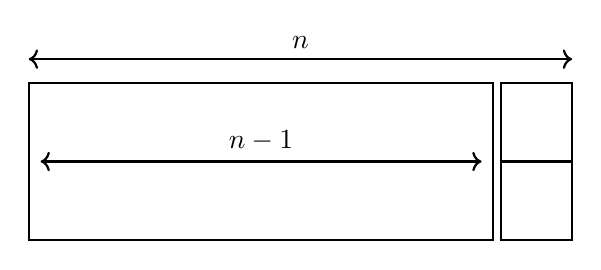
\begin{tikzpicture}
				\draw[thick] (0.05,0) rectangle (5.95,2);
				\draw[thick,<->] (0.2,1) -- (5.8,1) node[above, midway]{\(n-1\)};
				\draw[thick] (6.05, 0) rectangle (6.95, 2);
				\draw[thick] (6.05,1) -- (6.95,1);
				\draw[thick,<->] (0.05,2.3) -- (6.95,2.3) node[above, midway]{\(n\)};
			\end{tikzpicture}
			\caption{A board of size \(2 \times n\) made by appending a vertical \(2 \times 1\) tile to an arbitrary board of size \(2 \times (n-1)\).}
			\label{7b_1}
		\end{figure}

		Besides for these \(t_{n-1}\) ways, we also can exchange the last tile of any of the \(2 \times (n-1)\) sized boards which ended with a vertical \(2 \times 1\) tile with a \(2 \times 2\) tile or with two horizontal \(2 \times 1\) tiles. The number of such tiles which ended with a vertical \(2 \times 1\) tile is precisely the same as the number of tiles of size \(2 \times (n-2)\), since each of those was appended with a vertical tile to obtain a \(2 \times (n-1)\) sized tile. This is equal to \(t_{n-2}\). Since we can exchange any of these \(t_{n-2}\) tiles in two ways to form two distinct tilings, we must multiply \(t_{n-1}\) by two.

		Thus we have our recursive formula
		\begin{gather*}
			t_n = t_{n-1} + 2t_{n-2} \\
			t_0 = 1 \\
			t_1 = 1
		\end{gather*}
	\end{enumerate}

	\item[12.]
	\begin{enumerate}
		\item[(b)]
		We seek a closed form formula for the recursive formula
		\begin{gather*}
			a_n = 7a_{n-1} - 12a_{n-2} \\
			a_0 = 1 \\
			a_1 = 1
		\end{gather*}

		We begin by assuming a solution of the form \(x^n\), and substituting that into our recursive definition.
		\begin{align*}
			a_n &= x^n \\
			x^n &= 7x^{n-1} - 12x^{n-2} \\
			x^{n-2} \times x^2 &= x^{n-2} (7x - 12) \\
			x^2 &= 7x - 12 \\
			0 &= x^2 - 7x + 12 \\
			x &= \frac{7 \pm \sqrt{49 - 4 \times 12}}{2} \\
			&= 3 \text{ and } 4
		\end{align*}

		Now that we have solved the characteristic equation, we know that the closed form formula is of the form
		\[a_n = A \cdot 3^n + B \cdot 4^n\]

		Solving for \(A\) and \(B\) using the initial conditions we can obtain our closed form formula
		\begin{align*}
			1 &= A \cdot 3^0 + B \cdot 4^0 \\
			1 &= A \cdot 3^1 + B \cdot 4^1 \\
			A + B &= 1 \\
			3A + 4B &= 1 \\
			3A + 3B &= 3 \\
			B &= -2 \\
			A - 2 &= 1 \\
			A &= 3
		\end{align*}

		Finally, our closed form formula is
		\begin{align*}
			a_n &= 3 \cdot 3^n - 2 \cdot 4^n \\
				&= 3^{n+1} - 2^{2n+1}
		\end{align*}

		\item[(d)]
		Given the recursive formula below, a corresponding closed form formula must be found.
		\begin{gather*}
			a_n + 3a_{n-1} = 0 \\
			a_0 = -2
		\end{gather*}
		Rearranging the formula and expanding each term yields the following.
		\begin{align*}
			a_n &= -3a_{n-1} \\
			&= -3(-3a_{n-2}) \\
			&= (-3)^2(a_{n-2}) \\
			&= (-3)^2(-3a_{n-3}) \\
			&= (-3)^3(a_{n-3}) \\
			&= (-3)^3(-3a_{n-4}) \\
			&= (-3)^4(a_{n-4}) \\
			&\vdots \\
			&= (-3)^k(a_{n-k}) \\
			&\vdots \\
			&= (-3)^n(a_{n-n}) \\
			&= (-3)^n(a_{0}) \\
			&= (-3)^n(-2)
		\end{align*}

		Thus the closed form formula is
		\[a_n = -2(-3)^n\]
	\end{enumerate}

	\item[13.]
	\begin{enumerate}
		\item[(b)]
		The coefficient of the term
		\[x_1x_2{x_3}^2{x_4}^3\]
		in the expansion of
		\[(x_1+x_2+x_3+x_4)^7\]
		is equal to the multinomial coefficient
		\[\binom{7}{1, 2, 2, 3} = \frac{7!}{1! \times 2! \times 2! \times 3!} = \frac{5040}{24} = 210\]
	\end{enumerate}

\end{answers}

\end{document}
